%%%%%%%%%%%%%%%%%%%%%%%%%%%%%%%%%
% This is a slightly modified template of the one built by
% Steven V. Miller. Information can be found here:
%  http://svmiller.com/blog/2016/02/svm-r-markdown-manuscript/
%
% I added in a few other features.
%
% Here are the options that you can define in the YAML
% header.
%
% fontfamily - self-explanatory
% fontsize - self-explanatory (e.g. 10pt, 11pt)
% anonymous - true/false. If true, names will be supressed and the
%                       text will be double-spaced and ragged
%                       right with a separate page for title and abstract.
% endnotes - true/false. If true, the footnotes will be put in a
%                   section at the end just ahead of the references.
% endfloat - move all tables and figures to the end of the document
% keywords - self-explanatory
% thanks - shows up as a footnote to the title on page 1
% abstract - self explanatory
% appendix - if true, tables and figures will have  in
%                   front
% appendixletter - The letter to append to tables and figures in
%                             appendix
% pagenumber - Put in a number here to get a starting page number
%                         besides 1.
%%%%%%%%%%%%%%%%%%%%%%%%%%%%%%%%%%


\documentclass[11pt,]{article}
\usepackage[left=1in,top=1in,right=1in,bottom=1in]{geometry}
\usepackage{amsmath}
\usepackage{float}
\usepackage{dcolumn}
\usepackage{graphicx}

\newcommand*{\authorfont}{\fontfamily{phv}\selectfont}
\usepackage[]{mathpazo}


\usepackage[T1]{fontenc}
\usepackage[utf8]{inputenc}

\usepackage{abstract}
\renewcommand{\abstractname}{}    % clear the title
\renewcommand{\absnamepos}{empty} % originally center

\providecommand{\tightlist}{%
  \setlength{\itemsep}{0pt}\setlength{\parskip}{0pt}}

\renewenvironment{abstract}
 {{%
    \setlength{\leftmargin}{0mm}
    \setlength{\rightmargin}{\leftmargin}%
  }%
  \relax}
 {\endlist}

\makeatletter
\def\@maketitle{%
  \newpage
%  \null
%  \vskip 2em%
%  \begin{center}%
  \let \footnote \thanks
    {\fontsize{18}{20}\selectfont\raggedright  \setlength{\parindent}{0pt} \@title \par}%
}
%\fi
\makeatother




\setcounter{secnumdepth}{0}

\usepackage{longtable,booktabs}

\title{Patterns of Panethnic Intermarriage in the United States, 1980-2018  }



\author{\Large Aaron Gullickson\vspace{0.05in} \newline\normalsize\emph{University of Oregon, Sociology}  }


\date{}

\usepackage{titlesec}

\titleformat*{\section}{\large\bfseries}
\titleformat*{\subsection}{\normalsize\bfseries}
\titleformat*{\subsubsection}{\normalsize\itshape}
\titleformat*{\paragraph}{\normalsize\itshape}
\titleformat*{\subparagraph}{\normalsize\itshape}


\usepackage{natbib}
\setcitestyle{aysep={}}
\bibliographystyle{../../../paper/resources/ajs.bst}


%packages needed by kableExtra
\usepackage{booktabs}
\usepackage{longtable}
\usepackage{array}
\usepackage{multirow}
\usepackage{wrapfig}
\usepackage{float}
\usepackage{colortbl}
\usepackage{pdflscape}
\usepackage{tabu}
\usepackage{threeparttable}
\usepackage{threeparttablex}
\usepackage[normalem]{ulem}
\usepackage{makecell}
\usepackage{xcolor}

%\renewcommand{\refname}{References}
%\makeatletter
%\renewcommand\bibsection{
%    \section*{{\normalsize{\refname}}}%
%}%
%\makeatother

\newtheorem{hypothesis}{Hypothesis}
\usepackage{setspace}

\makeatletter
\@ifpackageloaded{hyperref}{}{%
\ifxetex
  \usepackage[setpagesize=false, % page size defined by xetex
              unicode=false, % unicode breaks when used with xetex
              xetex]{hyperref}
\else
  \usepackage[unicode=true]{hyperref}
\fi
}
\@ifpackageloaded{color}{
    \PassOptionsToPackage{usenames,dvipsnames}{color}
}{%
    \usepackage[usenames,dvipsnames]{color}
}
\makeatother
\hypersetup{breaklinks=true,
            bookmarks=true,
            pdfauthor={},
             pdfkeywords = {panethnicity; intermarriage; assortative mating, ethnic exogamy; immigration},
            pdftitle={Patterns of Panethnic Intermarriage in the United States, 1980-2018},
            colorlinks=true,
            citecolor=blue,
            urlcolor=blue,
            linkcolor=magenta,
            pdfborder={0 0 0}}
\urlstyle{same}  % don't use monospace font for urls

\usepackage{endnotes}


  \usepackage[notablist,nofiglist,noheads,tablesfirst]{endfloat}

\newlength{\normalparindent}
\setlength{\normalparindent}{\parindent}

%prettier captions for figures and tables
%I am making the text of figure captions smaller but not table captions
\usepackage[labelfont=bf,labelsep=period]{caption}
\captionsetup[figure]{font=footnotesize}

\begin{document}

% \pagenumbering{arabic}% resets `page` counter to 1
%


%\pagenumbering{gobble}

% \maketitle

{% \usefont{T1}{pnc}{m}{n}
\setlength{\parindent}{0pt}
\thispagestyle{plain}
{\fontsize{18}{20}\selectfont\raggedright
\maketitle  % title \par

}

{
   \vskip 13.5pt\relax \normalsize\fontsize{11}{12}
\hfill 

}

}







\begin{abstract}

    \hbox{\vrule height .2pt width 39.14pc}

    \vskip 8.5pt % \small

\noindent Intermarriage among ethnic groups belonging to the same panethnic category (e.g.~Asian, Latino) is thought to be an important indicator of the strength of panethnicity. Yet, most of the work on panethnic intermarriage uses older samples with significant data limitations. In this article, I use data on recently married couples from Census 1980 and the American Community Survey 2014-18 to analyze the likelihood of ethnic exogamy within the panethnic categories of Latino, East/Southeast Asian, and South Asian. I utilize a counterfactual marriage model that accounts for group size within local marriage markets, eliminates immigrants married abroad from analysis, and controls for birthplace and language endogamy. The results show that birthplace and language diversity are significant barriers to ethnic exogamy among Asians but not Latinos. Once birthplace and language endogamy are held constant, panethnic intermarriage is far more likely among Asians than among Latinos. East/Southeast Asian ethnic exogamy has increased over time, while Latino ethnic exogamy has not. Furthermore, East/Southeast Asian and South Asian intermarriage remains rare, suggesting that panethnic intermarriage among Asians occurs within two separate melting pots.


\vskip 8.5pt \noindent \emph{Keywords}: panethnicity; intermarriage; assortative mating, ethnic exogamy; immigration \par

    \hbox{\vrule height .2pt width 39.14pc}



\end{abstract}


\vskip 6.5pt

\noindent \newpage\doublespacing\raggedright\setlength{\parindent}{\normalparindent} \hypertarget{introduction}{%
\section{Introduction}\label{introduction}}

Social scientists have long treated patterns of intermarriage as a prime indicator of the underlying social distance and strength of boundaries separating groups. Because marriage is one of the most intimate kinds of social relationships, a widespread willingness to marry across group lines is seen as a key signifier that the salience of the boundaries separating those groups is weak \citep{gordon_assimilation_1964}.

An increase in intermarriage across one boundary is often treated as an indication that this boundary is dissolving or blurring, but it can also indicate a reshaping of existing boundaries. Widespread intermarriage among European ethnic groups in the mid-twentieth century contributed to the breakdown of salient ethnic divisions between these populations but also helped to re-consolidate a sense of collective whiteness \citep{lieberson_many_1988, alba_ethnic_1990, jacobsen_whiteness_1998}. Similarly, spurred by resurgent immigration to the US since the 1960s, intermarriage is seen as a key benchmark for gauging panethnic affinity among Asian and Latino ethnic groups today.\footnote{I use the term ``ethnic groups'' here to distinguish primarily different nationality groups among the Asian and Latino population, such as Chinese, Korean, Mexican, and Colombian. Ethnic differences can and do exist within the same nationality grouping, but are largely unmeasurable in the data that I use here.}

Panethnicity is defined by \citet{okamoto_panethnicity_2014a} as ``the construction of a new categorical boundary through the consolidation of ethnic, tribal, religious, or national groups.'' Within the larger theoretical tradition studying ethnoracial boundary formation, panethnicity is treated as a form of boundary expansion in which the salient boundary shifts from one level to another within a nested hierarchy of possible identification \citep{wimmer_making_2008}. From this boundary perspective, ethnoracial categories are not fixed, stable, or primordial, but can shift over time in response to historical events, as they have for the ethnoracial groups in the US today that we collectively view as White and Black. Understanding how such processes are playing out for contemporary Asian and Latino ethnic groups informs us about how social boundaries might shift in the future. Such shifts are consequential for issues of racial inequality, assimilation, political change, and even how we measure race and ethnicity itself.

The earliest work on panethnicity focused on collaboration among ethnically based organizations and movements \citep{lopez_panethnicity_1990, okamoto_theory_2003}. However, these authors also noted the importance of examining patterns of marriage to better understand ``interpersonal'' panethnicity \citep[pp.~167-168]{espiritu_asian_1993}. Early attempts to address this research question simply looked at outmarriage percentages which generally show the effects of group size more than underlying affinity \citep{shinagawa_asian_1996}. However, shortly after the turn of the century, several more sophisticated studies were published that generally found stronger evidence of panethnicity among Asians than Latinos \citep{qian_asian_2001, rosenfeld_salience_2001, qian_latinos_2004, fu_how_2007a, qian_crossing_2012}.

This prior work on intermarriage has contributed greatly to our understanding of the phenomenon of panethnicity, but is is also considerably out of date. Prior work used data from Census 1980, 1990, or 2000. The two later data sources have no information on marriage timing which limits researchers' ability to the identify and exclude immigrants married from analysis. Furthermore, much of the early work relies upon an examination of panethnicity among the relatively few Asian and Latino groups that were numerically large enough in historical data to sustain an analysis, while immigration from Asia and Latin America has diversified increasingly since this time.

In this article, I refresh our understanding of panethnic intermarriage using recent data from the 2014-2018 American Community Survey. I compare this data to Census 1980 data to analyze trends in panethnic intermarriage over time. Both of these data sources include timing of marriage which resolves several methodological difficulties with prior work. Additionally, I use a relatively novel counterfactual marriage model technique \citep{gullickson_counterfactual_2021} that allows me to easily adjust for differences in the spatial distribution of ethnic groups and to account for the role of birthplace and language endogamy when estimating the strength of panethnicity. Accounting for birthplace and language endogamy are critical for understanding patterns of panethnic intermarriage due to the considerable diversity in birthplace and language within and between Asian and Latino ethnic groups. Prior work has focused almost entirely on an immigrant-native comparison which does not adequately capture this complexity.

I find that patterns of panethnicity are very different for Asian and Latino ethnic groups. For Asians, panethnic affinity is very strong among East/Southeast Asian ethnic groups and among South Asian ethnic groups, but there is little evidence of panethnicity between South Asian and East/Southeast Asian ethnic groups. Furthermore, Asian panethnic intermarriage has also become more common over time. For Latinos, panethnic affinity is lower overall and in some cases is less likely than outmarriage to non-Latino racial groups. These different patterns have important implications for the future salience of panethnic categories.

\hypertarget{panethnicity-in-marriage}{%
\section{Panethnicity in Marriage}\label{panethnicity-in-marriage}}

Panethnic affinity may be driven by both cultural and structural factors \citep{lopez_panethnicity_1990}. Cultural factors such as shared language and religion may create affinity across ethnic or national boundaries. Structural factors such as economic and occupational similarity, spatial proximity, and the degree of racialization (the tendency of natives to treat all members of the panethnic category as a monolithic racial group) may also play a role in encouraging or discouraging panethnic affinity. The distinction between cultural factors and racialization has been particularly important in differentiating the experiences of Asians and Latinos. Latinos share cultural features such as language and religion that should promote panethnicity while Asians generally do not. On the other hand, racialization of Asians as a singular group tends to be stronger than for Latinos, who are more phenotypically diverse and racially ambiguous \citep{lopez_panethnicity_1990, kibria_construction_1997, qian_latinos_2004}.

Several important studies of panethnic intermarriage were performed shortly after the turn of the century, using data from the 1980 and 1990 US Census \citep{qian_asian_2001, rosenfeld_salience_2001, qian_latinos_2004, fu_how_2007a}. Both \citet{rosenfeld_salience_2001} and \citet{fu_how_2007a} explicitly compare the tendency toward panethnicity among Asians and Latinos and find a stronger tendency toward panethnicity among Asians. \citet{qian_asian_2001} and \citet{qian_latinos_2004} use similar methods to examine panethnicity among Asians and Latinos, respectively, and find substantial evidence of panethnic affinity, particularly among the native-born. Using slightly more recent data from Census 2000, \citet{qian_crossing_2012} estimated the likelihood of panethnic intermarriage for Mexicans, Puerto Ricans, Chinese, and Filipinos. Their results generally show similar levels of panethnicity across all four groups, and that panethnicity is most likely among the native-born and those immigrants who came to the US at an early age.

Some of these studies also compare how common interethnic marriage is in relation to interracial marriage with Whites and Blacks \citep{qian_asian_2001, fu_how_2007a, qian_crossing_2012}. In general, scholars have found that Asians are more likely to marry interethnically than to marry Whites or Blacks. Latinos are also much less likely to marry Blacks than to marry interethnically, but in some cases, depending on generation and the ethnic group under consideration, are more likely to marry Whites than to marry interethnically.

Although this prior work has enriched our understanding of panethnic intermarriage, it has also suffered from well-acknowledged methodological difficulties. All of the studies cited above use log-linear models to adjust for differences in group size. This approach allows scholars to properly estimate the underlying affinity between groups, apart from differential exposure to potential partners due to group size. However, basic log-linear models will not address differences in spatial settlement patterns among groups. Most individuals will find a partner within a local, rather than a national, context, and ethnoracial groups are not evenly distributed across the US. Without adjusting for these differences in geography, scholars will tend to underestimate the degree of ethnoracial exogamy \citep{harris_how_2005}. This issue is particularly problematic when studying panethnicity, because, although geographic dispersion is becoming more common, Latino and Asian ethnic groups have historically settled in different parts of the US \citep{massey_geographic_2008}. Some of the prior work on panethnicity has attempted to address this issue. \citet{fu_how_2007a} includes Census division as a parameter in log-linear models, while \citet{rosenfeld_salience_2001} estimated log-linear models separately within a few specific metropolitan areas. However, most of the prior work makes no adjustment for this important issue.

All work on intermarriage has to wrestle with the difference between measuring the prevalence and incidence of intermarriage. Ideally, scholars wish to capture the incidence of intermarriage by examining recently formed marriages. However, most large-scale data has lacked information on marriage timing and so scholars have had to resort to restricting the age of spouses to create semi-incidence measures with unknown biases.

When addressing intermarriage among Asians and Latinos, this limitation is compounded by the issue of immigrants married abroad (IMA). Without information on both the timing of marriage and the timing of immigration to the US, it is impossible to completely remove IMA from the analysis. Because IMA were mostly married in their country of origin, they will bias estimates toward ethnic endogamy \citep{hwang_problem_1990}. Researchers have used a variety of sample restrictions in an attempt to minimize this problem, but without information on marriage and migration timing, it cannot be fully eliminated.

A final issue in measuring panethnic intermarriage is the consideration of what ethnic groups to include. Historically, the most populous ethnic groups were Mexicans, Puerto Ricans, and Cubans among Latinos and Chinese, Filipino, Japanese, Korean, and Vietnamese among Asians. Prior work has focused on some subset of these groups because they are the numerically largest and because they can be clearly identified in earlier Census data. However, limiting analysis to only a few ethnic groups may distort the overall pattern of panethnic intermarriage.

Related to this issue, most prior work has not addressed the issue of South Asian panethnic intermarriage. The placement of South Asians within the panethnic category of Asian is contested at best. Individuals from the Indian subcontinent are treated as part of the panethnic Asian group by governmental agencies such as the Census Bureau, but research has shown that in everyday practice they are more generally treated as ``ambiguous non-whites'' \citep{kibria_not_1996, morning_racial_2001, schachter_finding_2014}. However, only \citet{qian_asian_2001} have analyzed panethnic intermarriage using data that includes South Asians. They found that Asian Indians had the lowest rate of intermarriage with other Asian groups.

\hypertarget{the-role-of-birthplace-and-language-endogamy}{%
\subsection{The Role of Birthplace and Language Endogamy}\label{the-role-of-birthplace-and-language-endogamy}}

Research on intermarriage is often framed around issues of assimilation and acculturation. Historically, intermarriage was seen as a key benchmark for assimilation into the ``mainstream'' culture \citep{gordon_assimilation_1964}. More recent work has problematized the assumption of one-way assimilation into the mainstream, most notably the work on segmented assimilation which suggests multiple pathways to assimilation for contemporary migrants \citep{portes_new_1993}.

Panethnicity has sometimes been framed as a pathway within the segmented assimilation approach, specifically as a form of ``selective acculturation'' \citep{bohra-mishra_intermarriage_2015}. However, this framing seems to deviate somewhat from the original idea of selective acculturation, in which an ethnic group engages in social closure to facilitate resource sharing and the intergenerational transfer of cultural meaning and identity. Panethnic intermarriage would work against such social closure.

Rather than treat panethnicity as a form of assimilation/acculturation, I treat it as a form of ethnoracial boundary expansion. Specifically, panethnicity is a form of ethnogenesis in which smaller minority groups are ``lumped'' together into larger minority categories \citep{kibria_construction_1997, wimmer_elementary_2008}. Such ethnogenesis can result from state efforts at consolidation, but can also arise from an increasing sense of solidarity and sense of linked fate among individuals in the lumped category \citep{wimmer_elementary_2008, okamoto_panethnicity_2014a}.

Ethnogenesis is not simply a function of assimilation and acculturation but can be deeply affected by cross-cutting trends related to these issues. Most notably, birthplace and language endogamy will present challenges to the likelihood of panethnic intermarriage in complex ways. Individuals will often prefer partners from the same birthplace due to the shared cultural understandings that arise from being born and raised in a particular place. Similarly, people are more likely to marry individuals who speak the same primary language because of ease of communication. We might expect birthplace endogamy to lower the likelihood of panethnicity for both Asians and Latinos, because all Asian and Latino ethnic groups have a substantial foreign-born sub-population and these members would prefer to marry someone from the same place of birth. On the other hand, language endogamy might affect Asian and Latino panethnic intermarriage differently, because Latino ethnic groups share a common language while Asian ethnic groups do not.

However, the actual effect of birthplace and language endogamy on panethnic intermarriage is considerably more complex than the simple expectations outlined above, because ethnic groups themselves are diverse in terms of birthplace and language. For example, among adults recently married or single in the 2014-18 American Community Survey data detailed below, 66\% of Japanese respondents spoke English as a primary language, while 41\% of Filipino respondents spoke English as a primary language. For those Japanese and Filipino individuals who both speak English, language endogamy will actually encourage panethnic intermarriage relative to ethnic endogamy with members of their own group who speak Japanese and Tagalog, respectively. Similarly, 31\% of Mexicans in the same sample spoke English as primary language, but only 13\% of Dominicans. In this case, however, the Mexicans and Dominicans who do not speak English typically both speak Spanish which will also encourage panethnic intermarriage when such potential partners are paired.

More broadly, in order for language and birthplace endogamy to serve as a barrier to panethnic intermarriage, the diversity in language and birthplace must be greater within the panethnic category than within the corresponding ethnic group. The strength of the barrier will depend on how much more diverse the panethnic category is than the ethnic group. This complex relationship has not been fully appreciated by prior work on the subject, which often addresses these issues simply by dividing the sample between the immigrant and native-born population.

Ideally, to estimate the underlying affinity for panethnic intermarriage, we want a model that can separate out those barriers to intermarriage resulting from language and birthplace endogamy. Such a model gives us a sense of how much panethnic intermarriage we would expect in a situation in which all Asians and Latinos are fully assimilated/acculturated to the US (i.e.~born in the US and speak English as their primary language).

In the analysis that follows, I address many of the weaknesses with prior data and models using a counterfactual marriage model to estimate the likelihood of panethnic intermarriage. The data from Census 1980 and the American Community Survey 2014-18 provide information on marriage timing which allows me to limit analysis to recent marriages while removing immigrants married abroad. The model framework allows me to account for differences in group size in local marriage markets while easily incorporating controls for birthplace and language endogamy. I use this model to compare trends in panethnic intermarriage for Latinos, East/Southeast Asians, and South Asians.

\hypertarget{data-and-methods}{%
\section{Data and Methods}\label{data-and-methods}}

The data for this analysis are derived from the microdata sample of the 1980 US Census and the American Community Survey (ACS) for 2014-2018. The ACS is an annual 1-in-100 survey of the United States population, conducted by the United States Census Bureau. The 1980 US Census is the last Census dataset to include information about marriage timing, before it was re-included on the 2008 ACS. To increase sample size for smaller ethnoracial categories, I pool five years of ACS data from 2014-2018. Both data sources were extracted from the Integrated Public Use Microdata Series (IPUMS) system \citep{ruggles_ipums_2020}.

In both data sources, I restrict the analysis to all opposite-sex marriages formed in the previous five years that were a first marriage for both partners. The restriction to opposite-sex first marriages is necessary for comparison because the Census 1980 only recorded marriage timing relative to first marriage and does not include same-sex unions. To avoid capturing marriages occurring in different local contexts, I also remove marriages in which at least one of the partners migrated to the US or across state lines in the last five years.

I use a counterfactual marriage model \citep{qian_marriage_2018, gullickson_counterfactual_2021} to measure the likelihood of panethnic intermarriage. For each marriage, I construct a choice set of one real union and twenty fictional unions. Fictional unions are created by sampling alternate partners for one randomly determined spouse from a pool of potential partners. I then use a conditional logit model to predict how partner characteristics relate to the likelihood of observing the true union, as follows: 
\begin{equation}
P_{ij}=\frac{e^{\mathbf{x}_{ij}\beta}}{\sum_{k=1}^J e^{\mathbf{x}_{ik}\beta}}
\end{equation}
where \(P_{ij}\) is the probability that union \(j\) within choice set \(i\) is the actual union. \(J\) is the total number of unions in the choice set. The vector \(\mathbf{x}_{ij}\) defines the characteristics of the union and the \(\beta\) vector provides estimated log-odds ratios indicating how the odds of an actual union change with \(\mathbf{x}_{ij}\). The model is estimated as a fixed-effects logistic regression model with fixed effects for each choice set.

The set of potential alternate partners from which fictional spouses are sampled is made up of all unmarried adults as well as individuals who were married in the previous five years, with the restriction that all alternate partners must not nave migrated to the US or across state lines in the last five years. To better capture local marriage market context, alternate partners are sampled from among individuals residing in the same metropolitan area of residence when this can be identified for a respondent, and otherwise by the state of residence. Metropolitan area is not directly identifiable in the data used here due to confidentiality concerns, but can be deduced for many metropolitan areas based on the finest geographic identifier of the respondent (county group in Census 1980 and Public Use Microdata Area, or PUMA, in the ACS). IPUMS provides metro area identification for respondents in cases where the county group or PUMA was mostly contained within the metropolitan area. Figure \ref{fig:metro-areas} shows the identifiable metropolitan areas used in the analysis for both time periods. Although not all metropolitan areas are identified in the data, most major metropolitan areas are included in both time periods. Coverage differs somewhat by period, with more extensive coverage in the later time period.

\begin{figure}
\centering
\includegraphics{/Users/aarong/Research/Projects/panethnicity_intermar/analysis/output/msa_map.pdf}
\caption{\label{fig:metro-areas}Metropolitan statistical areas identifiable in the data by data source. The darkest shade indicates overlapping areas in the two data sources.}
\end{figure}

Because this approach relies upon a random sample of alternate partners, results will vary each time this sampling procedure is performed. To account for the added uncertainty due to sampling, I perform the sampling procedure separately three times to produce three separate analytical datasets. I then run parallel models on all three datasets and pool \(\beta\) estimates and standard errors using the same methods as those employed for multiple imputation \citep{rubin_multiple_1987, gullickson_counterfactual_2021}.

\hypertarget{variable-construction}{%
\subsection{Variable Construction}\label{variable-construction}}

One advantage of the counterfactual marriage model is that it allows for the easy incorporation of a variety of quantitative and categorical variables. I utilize that feature to account for age differences, educational differences, birthplace endogamy, and language endogamy when estimating the likelihood of panethnic intermarriage.

I measure ethnoracial categories by a combination of the race and Hispanicity questions in both data sources. Table \ref{tab:sample-size-table} shows the sample size for all ethnoracial groups included in the analysis. I classify non-Asian and non-Latino respondents as White, Black, or American Indian/Alaska Native (AIAN). Due to small sample size, I exclude Pacific Islanders, multiracial respondents, and non-Latino others from the analysis. The race question includes several Asian nationalities (e.g.~Chinese, Korean, Filipino) as well as a write-in response for ethnic/national identities not captured by the existing categories. Similarly, the Hispanicity question includes major Latino ethnic groups (e.g.~Mexican, Puerto Rican, Cuban) as well as a write-in option. Importantly, the Census 1980 data includes a far more limited set of identifiable ethnic groups for both Asians and Latinos than the ACS data. In Census 1980, I can only identify Mexicans, Puerto Ricans, and Cubans among Latinos and Chinese, Japanese, Korean, Filipino, Vietnamese, and Asian Indian respondents among Asians. To address this restriction, I estimate two different kinds of models for the ACS data. In the first model, I restrict the data only to those ethnic groups that were available in the Census 1980 data to allow more direct comparison over time. I also estimate models using the full ACS data to explore how using a broader set of ethnic groups changes our understanding of panethnicity, but these models are not directly comparable to the Census 1980 models.

\begin{table}

\caption{\label{tab:sample-size-table}Sample size of marriages and alternate partners by data source and ethnoracial category.}
\centering
\begin{tabu} to \linewidth {>{\raggedright\arraybackslash}p{6.5cm}>{\raggedleft}X>{\raggedleft}X}
\toprule
Category & Census 1980 & ACS 2014-2018\\
\midrule
\addlinespace[0.3em]
\multicolumn{3}{l}{\textbf{Marriages}}\\
\hspace{1em}Marriages in the previous five years & 285,523 & 503,348\\
\addlinespace[0.3em]
\multicolumn{3}{l}{\textbf{Alternate Partners}}\\
\hspace{1em}White & 2,926,629 & 4,368,640\\
\hspace{1em}Black & 535,993 & 887,837\\
\hspace{1em}American Indian/Alaska Native & 24,304 & 73,760\\
\hspace{1em}Latino & 162,526 & 859,250\\
\hspace{1em}\hspace{1em}Mexican & 113,648 & 560,124\\
\hspace{1em}\hspace{1em}Puerto Rican & 35,444 & 97,695\\
\hspace{1em}\hspace{1em}Cuban & 13,434 & 39,473\\
\hspace{1em}\hspace{1em}Salvadorian &  & 32,947\\
\hspace{1em}\hspace{1em}Dominican &  & 29,201\\
\hspace{1em}\hspace{1em}Guatemalan &  & 19,449\\
\hspace{1em}\hspace{1em}Colombian &  & 18,826\\
\hspace{1em}\hspace{1em}Honduran &  & 11,926\\
\hspace{1em}\hspace{1em}Peruvian &  & 10,548\\
\hspace{1em}\hspace{1em}Ecuadorian &  & 10,226\\
\hspace{1em}\hspace{1em}Nicaraguan &  & 7,605\\
\hspace{1em}\hspace{1em}Argentinian &  & 4,619\\
\hspace{1em}\hspace{1em}Venezuelan &  & 4,404\\
\hspace{1em}\hspace{1em}Panamanian &  & 3,960\\
\hspace{1em}\hspace{1em}Chilean &  & 2,531\\
\hspace{1em}\hspace{1em}Costa Rican &  & 2,399\\
\hspace{1em}\hspace{1em}Bolivian &  & 1,814\\
\hspace{1em}\hspace{1em}Uruguayan &  & 1,046\\
\hspace{1em}\hspace{1em}Paraguayan &  & 457\\
\hspace{1em}East and Southeast Asian & 30,432 & 199,180\\
\hspace{1em}\hspace{1em}Chinese & 9,980 & 63,621\\
\hspace{1em}\hspace{1em}Filipino & 6,557 & 48,254\\
\hspace{1em}\hspace{1em}Vietnamese & 331 & 29,119\\
\hspace{1em}\hspace{1em}Korean & 2,066 & 24,163\\
\hspace{1em}\hspace{1em}Japanese & 11,498 & 15,023\\
\hspace{1em}\hspace{1em}Cambodian &  & 4,880\\
\hspace{1em}\hspace{1em}Hmong &  & 4,563\\
\hspace{1em}\hspace{1em}Laotian &  & 3,762\\
\hspace{1em}\hspace{1em}Thai &  & 3,429\\
\hspace{1em}\hspace{1em}Burmese &  & 1,156\\
\hspace{1em}\hspace{1em}Indonesian &  & 980\\
\hspace{1em}\hspace{1em}Malaysian &  & 230\\
\hspace{1em}South Asian & 2,882 & 41,222\\
\hspace{1em}\hspace{1em}Asian Indian & 2,882 & 34,446\\
\hspace{1em}\hspace{1em}Pakistani &  & 4,785\\
\hspace{1em}\hspace{1em}Bangladeshi &  & 1,402\\
\hspace{1em}\hspace{1em}Sri Lankan &  & 589\\
\bottomrule
\end{tabu}
\end{table}

I model panethnic and racial intermarriage using a set of gender-symmetric dummy variables where the reference category is an ethnoracially endogamous union (e.g.~a White-White or Chinese-Chinese marriage). Because the number of ethnoracial categories is large, modeling every possible combination of these categories for exogamous unions is not feasible. In my most restrictive models, I apply two limits on the parameterization that make model estimation possible. First, when analyzing intermarriage with Whites, Blacks, and American Indians/Alaska Natives, I group Asian and Latino ethnic groups into the larger panethnic categories of Latino, East/Southeast Asian, and South Asian. For example, a union involving a Black and Mexican partner and a union involving a Black and Colombian partner would both be coded as a Black-Latino union. Second, I model the likelihood of panethnic intermarriage using three dummy variables to indicate any form of ethnic exogamy within the three panethnic categories of Latino, East/Southeast Asian, and South Asian. For example, a union involving a Chinese and Japanese partner and a union involving a Korean and Filipino partner would both be coded as East/Southeast Asian ethnic exogamy. This approach allows me to estimate the average likelihood of ethnic exogamy across all possible combinations, but does not capture particular affinities of disaffinities among ethnic groups within the panethnic category. I partially relax both of these assumptions in later models of the ACS data.

Because I separate South Asian from East/Southeast Asian groups and only Asian Indians are identifiable in the Census 1980 data, I cannot estimate panethnic parameters over time for South Asians. Thus, when analyzing change over time, I focus exclusively on East/Southeast Asians and Latinos.

I account for language and birthplace endogamy with simple dummy variables indicating whether the two potential partners share the same primary language or birthplace, respectively. Primary language is determined by what language the respondent reported speaking at home. Because this variable is measured after a marriage has occurred, it may somewhat overestimate language endogamy among respondents. Some partners who spoke different languages when they met may have shifted the language spoken at home after marriage.

Birthplace endogamy is complicated by the ``1.5'' generation -- individuals who were born outside of the United States but migrated as children and whose formative experiences are partially defined by acculturation within the US. I consider three possibilities for coding the birthplace endogamy of such individuals, organized by the assumed degree of acculturation. First, such individuals could be considered birthplace endogamous only with a person from the same actual birthplace. Second, such individuals could be considered birthplace endogamous with either a person from their actual birthplace or a person born in the USA. Third, such individuals could be considered only birthplace endogamous with a person born in the USA.

To test the accuracy of these three scenarios, I fit models using each coding scheme to the Census 1980 and full ACS data. Following \citet{rumbaut_ages_2004a}, I also divide the 1.5 generation into a ``1.75'' generation (those who arrived in the US before the age of 6), a ``1.5'' generation (those who arrived in the US between the ages of 6-12), and a ``1.25'' generation (those who arrived in the US between the ages of 13-17). For these three groups, I consider every possible combination of coding such that earlier generations are not more acculturated than later generations (e.g.~the 1.25 generation could not be ``both'' in cases where the 1.5 generation is ``birthplace only''). Table \ref{tab:deviance-bendog} below shows the model fit of all ten possible combinations for both data sources. Model fit is shown by deviance, where lower deviance indicates better fit.

\begin{table}

\caption{\label{tab:deviance-bendog}Model fit to Census 1980 and ACS data using different specifications of birthplace endogamy for 1.25, 1.5, and 1.75 generations. Minimum deviance is shown in bold.}
\centering
\begin{tabu} to \linewidth {>{\raggedright}X>{\raggedright}X>{\raggedright}X>{\raggedleft}X>{\raggedleft}X}
\toprule
\multicolumn{3}{c}{Generation} & \multicolumn{2}{c}{Model Deviance} \\
\cmidrule(l{3pt}r{3pt}){1-3} \cmidrule(l{3pt}r{3pt}){4-5}
1.75 & 1.5 & 1.25 & Census 1980 & ACS 2014-18\\
\midrule
Birthplace & Birthplace & Birthplace & \textbf{1,122,736} & 1,850,594\\
Both & Birthplace & Birthplace & 1,122,758 & 1,849,753\\
USA & Birthplace & Birthplace & 1,122,856 & 1,850,491\\
Both & Both & Birthplace & 1,122,775 & \textbf{1,849,202}\\
USA & Both & Birthplace & 1,122,851 & 1,849,714\\
USA & USA & Birthplace & 1,123,002 & 1,851,089\\
Both & Both & Both & 1,122,932 & 1,850,676\\
USA & Both & Both & 1,122,968 & 1,850,894\\
USA & USA & Both & 1,123,013 & 1,851,576\\
USA & USA & USA & 1,122,968 & 1,852,855\\
\bottomrule
\multicolumn{5}{l}{\rule{0pt}{1em}\textit{Notes: }}\\
\multicolumn{5}{l}{\rule{0pt}{1em}Age of US arrival by generation is 0-5 (1.75), 6-12 (1.5), and 13-17 (1.25). All models include}\\
\multicolumn{5}{l}{\rule{0pt}{1em}controls for educational differences, age differences, ethnoracial endogamy, and language}\\
\multicolumn{5}{l}{\rule{0pt}{1em}endogamy.}\\
\end{tabu}
\end{table}

For both time periods, the most preferred models use birthplace only coding for those respondents who entered the US after age 12. The USA only option representing full acculturation was not preferred for any group in either time period. In the Census 1980 data, the most preferred model treated all three groups as first generation individuals. The more recent ACS data preferred a model in which both the 1.75 and 1.5 generations were considered birthplace endogamous with partners either from the actual birthplace or the USA. The shift over time suggests greater acculturation of the 1.5 and 1.75 generation today than in 1980. For all models in the analysis that follows, I code birthplace endogamy according to the best-fitting model for each data source from Table \ref{tab:deviance-bendog}.

All models used here include controls for age and educational differences between potential partners. Age differences are modeled by taking the numerical age difference between partners and its square. Educational differences are modeled using educational crossing parameters \citep{schwartz_trends_2005}. All respondents are categorized as having less than a high school diploma, a high school diploma, some college education, or at least a four-year college degree. Three dummy variables indicate whether a particular union involves crossing the adjacent pairwise boundaries between these four categories. Results are cumulative such that a marriage involving one partner with less than a high school education and one partner with a four-year college degree would require passing all three boundaries. I also include parameters that measure the likelihood of female educational hypergamy (marrying higher in education) and female educational hypogamy (marrying lower in education).

In the results below, I use graphical visualizations to present important results from the models. In all cases, results are presented as the ratio of the odds of a particular kind of exogamy (racial or ethnic) to the odds of ethnoracial endogamy. An odds ratio of one indicates no barrier to a given kind of exogamy. The full model results upon which figures are based are available in tabular form in the supplementary materials for this article.

\hypertarget{results}{%
\section{Results}\label{results}}

\hypertarget{birthplace-and-language-diversity}{%
\subsection{Birthplace and Language Diversity}\label{birthplace-and-language-diversity}}

Before moving to the model results, I first show the complex ways in which birthplace and language endogamy affect the likelihood of panethnic intermarriage. I use the Blau index \citep{blau_inequality_1977} to measure language/birthplace diversity within each Asian and Latino ethnic group and to measure diversity within each panethnic category. The Blau index of diversity (\(D\)) is calculated as: 
\begin{equation}
D=1-\sum_{i=1}^R p_i^2 
\end{equation} 
where \(p_i\) is the proportion of the total population belonging to group \(i\) and \(R\) is the total number of groups. The Blau index has an intuitively appealing interpretation as the probability that two randomly drawn members from the population belong to the same group.

\begin{figure}
\centering
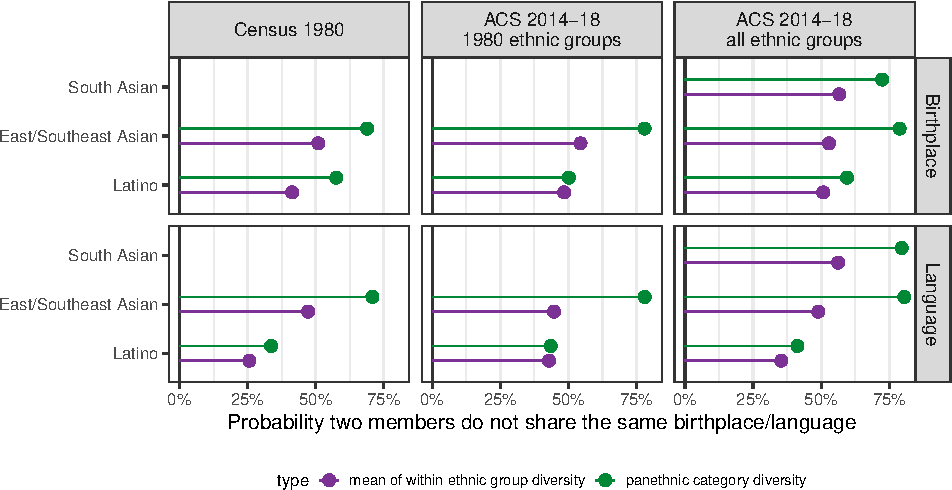
\includegraphics{main_files/figure-latex/diversity-pan-bar-1.pdf}
\caption{\label{fig:diversity-pan-bar}Birthplace and language diversity within Asian and Latino ethnic groups and panethnic categories. Diversity is measured by the Blau index which gives the probability that two randomly selected members of the group do not share the same birthplace/language. Results are based upon alternate partners from each data source.}
\end{figure}

Figure \ref{fig:diversity-pan-bar} shows the Blau index for language and birthplace across East/Southeast Asian, South Asian, and Latino ethnic and panethnic categories, using data on alternate partners in the two time periods. To simplify presentation, I take the mean diversity within each specific ethnic group and compare this directly to the diversity across the panethnic category as a whole. The likelihood of panethnic intermarriage will be reduced in cases where panethnic diversity is greater than average diversity within ethnic groups.

Significant language and birthplace diversity is observable within specific ethnic groups. For example, the average diversity in birthplace within specific Latino ethnic groups in the ACS data is nearly 60\%, indicating that two randomly determined members of the same ethnic group would not share the same birthplace about 60\% of the time.

Although this within ethnic group diversity is substantial, panethnic diversity in language and birthplace is greater than within ethnic group diversity for all three panethnic categories in both time periods. However, these differences are small for Latinos, while they are quite large for Asians. Because Latinos share a common language, this result was expected for language, but I also observe a similar pattern for birthplace. What differences exist among Latino ethnic groups have also diminished over time, whereas they have grown for East/Southeast Asians.

Overall, Figure \ref{fig:diversity-pan-bar} shows that language and birthplace endogamy are important barriers to panethnic intermarriage among Asians, but play little role in panethnic intermarriage among Latinos. With that in mind, I now turn to models that estimate the likelihood of panethnic intermarriage with and without accounting for birthplace and language endogamy.

\hypertarget{modeling-panethnicity}{%
\subsection{Modeling Panethnicity}\label{modeling-panethnicity}}

Figure \ref{fig:exog-lolly} shows the estimated odds of ethnic exogamy relative to ethnic endogamy for all three panethnic categories in both time periods. As these odds ratios approach one, the odds of ethnic exogamy (e.g.~a Chinese person marrying a Japanese person) increase relative to ethnic endogamy (e.g.~a Japanese person marrying a Japanese person).

\begin{figure}
\centering
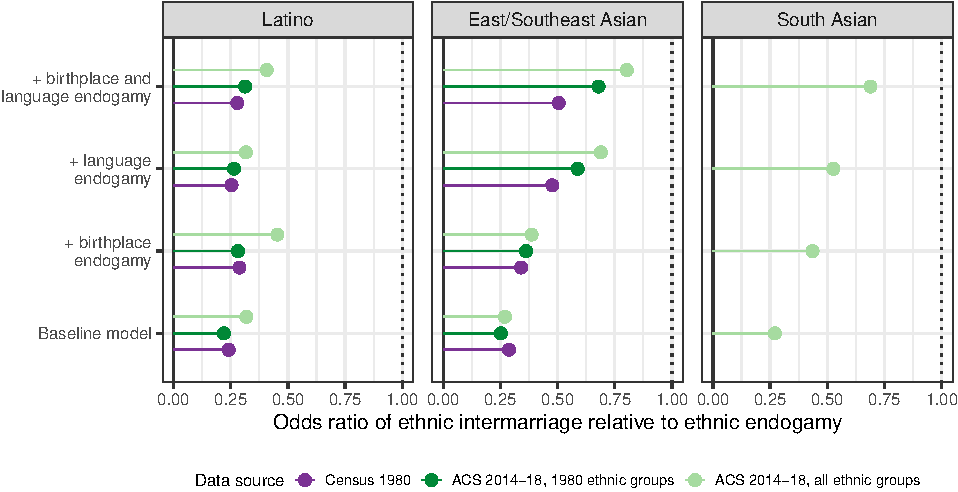
\includegraphics{main_files/figure-latex/exog-lolly-1.pdf}
\caption{\label{fig:exog-lolly}The odds of ethnic exogamy for Latinos, East/Southeast Asians, and South Asians over time and model specification. The baseline model controls for age and educational differences.}
\end{figure}

The baseline model includes only controls for age and educational differences between potential partners. I then include birthplace and language endogamy separately and together to determine the effects of these variables individually and collectively on the odds of ethnic exogamy.

In the baseline model, the odds of ethnic exogamy are similar for all three groups. In all cases, ethnic exogamy is about 25\% as likely as ethnic endogamy. The results also show a very slight decline in the odds of ethnic exogamy from 1980 to 2014-2018 when restricting to ethnic groups that were available in the 1980 data.

For Latinos, controlling for birthplace and language endogamy increases the overall odds of ethnic exogamy only very slightly, with birthplace endogamy having a slightly larger effect. Overall, however, the odds are hardly changed at all. Furthermore, there is no evidence of change across the two time periods when limiting the analysis to comparable ethnic groups.

For both Asian panethnic categories, controlling for birthplace and language endogamy substantially increases the odds of ethnic exogamy, to the point that ethnic exogamy in the later time period is not unusual. In the ACS data, the odds of ethnic exogamy are roughly 75\% as high as the odds of ethnic endogamy for both East/Southeast Asians and South Asians once I control for both language and birthplace endogamy. Controlling for language endogamy produces larger changes than controlling for birthplace endogamy, but both variables play a role. The odds of ethnic exogamy for East/Southeast Asians have also increased over time in models that account for birthplace and language endogamy. Using comparable ethnic groups, the odds of ethnic exogamy for East/Southeast Asians were about half those of ethnic endogamy in 1980, but have grown to nearly 75\% by the more recent time period.

For both Latinos and East/Southeast Asians, ethnic exogamy is more likely in models that include all ethnic groups from the ACS data rather than just the groups that were available in the Census 1980 data. These results suggest greater ethnic exogamy among these more recent and smaller groups. The overall effects of birthplace and language endogamy on ethnic exogamy are the same in these models using the expanded ethnic group data.

Figure \ref{fig:exog-lolly} shows the important role that birthplace and language endogamy play in panethnic intermarriage. In actuality, we observe similar odds of ethnic exogamy among Asians and Latinos. However, the low odds of ethnic exogamy for Asians are largely a function of the high level of diversity in birthplace and language between Asian ethnic groups. These barriers do not exist for Latinos. Controlling for these factors reveals a stronger affinity for panethnicity among Asian than Latinos in the absence of birthplace and language barriers.

Figure \ref{fig:changes-intermar} shows the odds of East/Southeast Asian and Latino ethnic exogamy in comparison to the odds of interracial marriage more broadly. All results in Figure \ref{fig:changes-intermar} are from the model that accounts for birthplace and language endogamy. East/Southeast Asian ethnic exogamy stands out as far more likely than any form of interracial marriage. Latino ethnic exogamy, on the other hand, is comparable in likelihood to several forms of interracial marriage. When limiting the analysis to comparable ethnic groups over time, White-Latino intermarriage was less likely than Latino ethnic exogamy in 1980, but has increased in frequency substantially and is now slightly more likely than Latino ethnic exogamy in the more recent time period. When the analysis is expanded to all Latino ethnic groups, Latino ethnic exogamy is sightly more likely than White-Latino exogamy, but the magnitudes are similar.

\begin{figure}
\centering
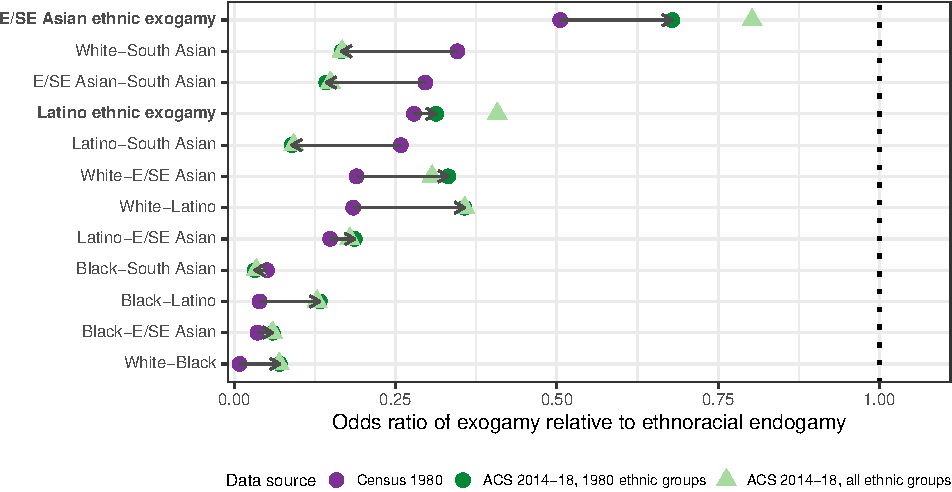
\includegraphics{main_files/figure-latex/changes-intermar-1.pdf}
\caption{\label{fig:changes-intermar}Odds of ethnoracial exogamy relative to endogamy across two time periods. Results are based on models that control for age differences, educational differences, and birthplace and language endogamy. Values are sorted by ethnoracial exogamy in 1980. Arrows show the change across the two time periods based on comparable sets of ethnic groups. Results for American Indian/Alaska Native intermarriage are excluded due to sampling variability.}
\end{figure}

Figure \ref{fig:changes-intermar} also shows the results for South Asian interracial marriage over time. The results show significant declines in South Asian interracial marriage with all other groups over the time period. These results, however, should probably be viewed with caution. In the earlier time period, the only South Asian group available was ``Asian Indian'' and research has shown that respondents sometimes confuse the categories of ``Asian Indian'' and ``American Indian'' in race responses \citep{liebler_american_2004}. Given the novel character of the ``Asian Indian'' category in 1980, it is likely that such misreporting has gone down over time. This may contribute to the overall decline in interracial marriage over time, if American Indians are less endogamous, on average, than Asian Indians.\footnote{Although not shown here, I also found that the odds of intermarriage between American Indian/Alaska Natives and South Asians was roughly 1.9 to 1 in 1980 but declined to 0.103 to 1 in the later ACS data. This result suggests that such race reporting errors played a greater role in 1980 than the later data.} Nonetheless, the results here show a relatively low odds of intermarriage between South Asians and East/Southeast Asians in both time periods, suggesting that Asian panethnicity occurs within two separate ``melting pots'' for South Asians and all other Asian ethnic groups.

Figure \ref{fig:changes-intermar} also documents that the lowest likelihood of intermarriage in both time periods is that between Blacks and all other groups, despite some substantial increases in these odds. These results highlight the enduring strength of the Black/non-Black boundary in the US despite increasing diversity in the overall population.

\hypertarget{group-specific-affinities}{%
\subsection{Group-Specific Affinities}\label{group-specific-affinities}}

The preceding models used a single ethnic exogamy term for each panethnic category such that the odds of ethnic exogamy are assumed to be the same regardless of which specific groups are paired. For example, the odds of ethnic exogamy into a Japanese-Korean union would be the same as those for a Japanese-Filipino union. I now turn to models of the ACS data that relax this assumption and allow the estimation of specific affinities within the matrix of ethnic groups that make up the three panethnic categories.

If I considered every possible combination within panethnic categories in the ACS data, I would need to replace my three ethnic exogamy terms with 243 group specific parameters. Given that some of these groups are quite small in the dataset, models could not be fit to this fully expanded set, due to issues with sparseness and model convergence. I experimented with the largest possible set of ethnic groups for which I could reliably fit data and found that this model included the five East/Southeast Asian ethnic groups available in the Census 1980 data (Chinese, Filipino, Vietnamese, Korean, and Japanese) and the ten largest Latino groups, with the exception of Hondurans. I could not fit ethnicity specific models for South Asians because of the small size of non-Asian Indian groups in the South Asian category .

In addition to separate parameters for each specific pairing of ethnic exogamy, I also include ethnic group specific parameters for intermarriage with Whites and Blacks. These parameters allow me to examine variation for each specific ethnic group in the tendency to intermarry with Whites and Blacks.

Figure \ref{fig:ethnic-heat-map} shows the group-specific odds of ethnic exogamy for the five East/Southeast Asian ethnic groups and the nine Latino ethnic groups, based on these models. I also provide a dendrogram that indicates the relative distance between each of these ethnic groups based on a tree diagram. The dendrogram is calculated by treating the inverse of the odds ratio as a measure of distance and measuring unweighted average distances.

\begin{figure}
\centering
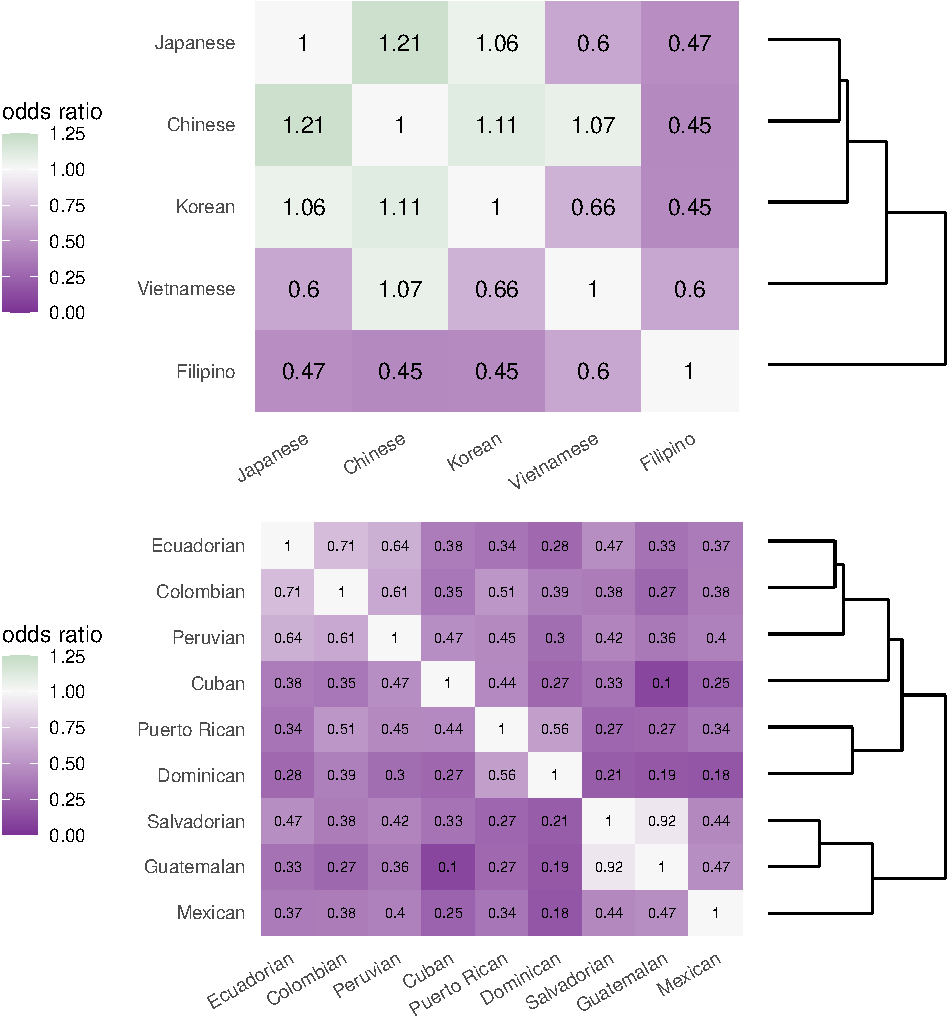
\includegraphics{main_files/figure-latex/ethnic-heat-map-1.pdf}
\caption{\label{fig:ethnic-heat-map}Odds of ethnic exogamy relative to ethnic endogamy between ethnic groups in ACS 2014-2018 data. The upper panel shows East/Southeast Asian ethnic groups and the lower panel shows Latino ethnic groups. Dendrograms on the right are based on hierarchical clustering using unweighted average distances where distance was measured by the inverse of these odds ratios. Results are based on models that control for age differences, education differences, and language and birthplace endogamy.}
\end{figure}

The top panel of figure \ref{fig:ethnic-heat-map} shows no social distance between the three East Asian groups of Chinese, Korean, and Japanese. The point estimates actually suggest that, holding language and birthplace endogamy constant, the odds of ethnic exogamy are slightly higher than ethnic endogamy among these groups. However, none of these odds ratios are statistically distinguishable from one using a p-value cutoff of 0.05.

Social distance remains between these East Asian groups and the Vietnamese and Filipino ethnic groups, with the exception of the Vietnamese-Chinese case for which there is no barrier to ethnic exogamy. These results suggest some regional distinction in panethnic intermarriage among East/Southeast Asians. Filipinos, in particular, have the lowest odds of ethnic exogamy with all of the other Asian groups, suggesting a stronger boundary separating Filipinos from wider East/Southeast Asian panethnicity. This may reflect the unique Spanish cultural inheritance of the Philippines. To more formally test this hypothesis, I included a specific dummy variable for Latino-Filipino intermarriage and found that the odds of Latino-Filipino intermarriage were about double the odds of intermarriage between Latinos and other East/Southeast Asian groups.

The bottom panel of figure \ref{fig:ethnic-heat-map} shows comparable results for the nine Latino ethnic groups. Overall, the odds ratios here are much lower than those for Asian ethnic groups, reflecting the overall lower ethnic exogamy among Latinos. The only case with no evidence of barriers to ethnic exogamy was for Salvadorians and Guatemalans, where the estimated odds ratio is close to one.

Affinities between Latino ethnic groups tend to cluster by region, with higher odds of intermarriage within the three groups of South American, Caribbean, and Central American/Mexican nationalities. The one exception to this pattern is for Cubans, who tend to be about equal distance from both the South American and Caribbean groupings.

Figure \ref{fig:racial-exogamy} shows the odds of intermarriage with Whites and Blacks for each of the East/Southeast Asian and Latino ethnic groups. For comparison, all of the ethnic exogamy odds ratios for a given ethnic group are also shown with small grey dots.

\begin{figure}
\centering
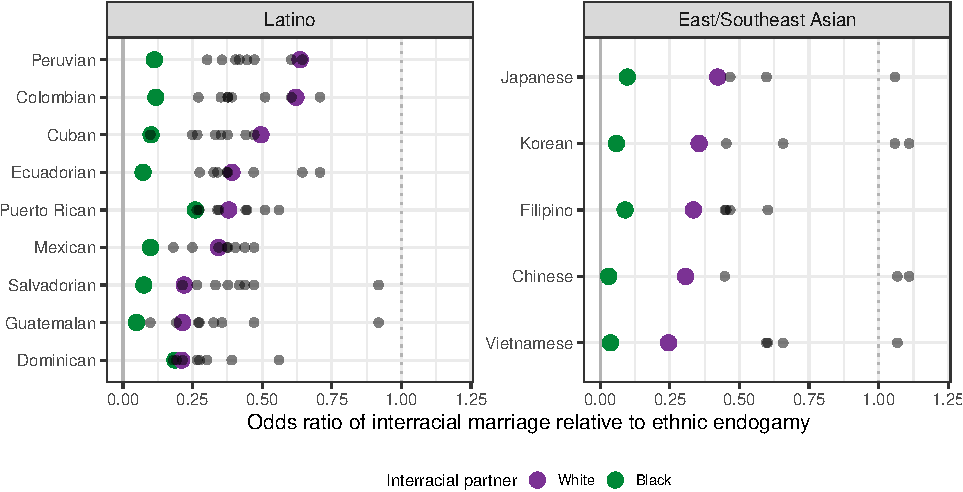
\includegraphics{main_files/figure-latex/racial-exogamy-1.pdf}
\caption{\label{fig:racial-exogamy}Odds of interracial marriage with Whites and Blacks for major Latino and East/Southeast Asian ethnic groups. For reference, odds of ethnic exogamy to other major ethnic groups are shown by small grey dots. Models are sorted based on the odds ratio of intermarriage with Whites. All models control for age differences, education differences, and language and birthplace endogamy.}
\end{figure}

The variation in the likelihood of interracial marriage across ethnic groups is more pronounced for Latino ethnic groups than for East/Southeast Asian groups. Among Latinos, Peruvians and Colombians are the most likely to intermarry with Whites with an odds about 60\% as high as ethnic endogamy. At the other end of the spectrum the odds of Dominican-White intermarriage are just under 25\% as likely as ethnic endogamy. For the five East/Southeast Asian groups, the odds ratios range from about 25\% to 42\%.

For all East/Southeast Asian and Latino ethnic groups, intermarriage with Whites is more likely than intermarriage with Blacks. The odds of intermarriage with Blacks are uniformly low for all five East/Southeast Asian groups. The odds of intermarriage are also low for most Latino groups, with the exception of Dominicans and Puerto Ricans. For Dominicans, the odds of intermarriage with Blacks are almost identical to the odds of intermarriage with Whites. For Puerto Ricans, the odds of intermarriage with Blacks are the highest of any Latino ethnic group and only slightly less likely than the odds of intermarriage with Whites. These differences almost certainly reflect the much higher prevalence of Afrodescent in Puerto Rican and Dominican populations and the racialization of members of these populations as Black within the US.

The relative placement of ethnic exogamy odds ratios for each ethnic group in Figure \ref{fig:racial-exogamy} is also telling. For all five Asian ethnic groups, every ethnic exogamy parameter is greater than the odds of intermarriage with Whites. For the Latino groups, these ethnic exogamy parameters are frequently in between the odds of White and Black intermarriage. For example, both Peruvians and Cubans are more likely to outmarry to a White person than to intermarry with any of the other Latino groups here. Mexicans are only slightly more likely to outmarry to most other Latino ethnic groups as they are to Whites, and are substantially less likely in two cases (Dominicans and Cubans).

Overall, Figure \ref{fig:racial-exogamy} implies very different patterns of intermarriage for Latino and East/Southeast Asian ethnic groups. East/Southeast Asian ethnic groups follow the same general pattern. Panethnic intermarriage is more likely than intermarriage with Whites or Blacks, and the barriers to intermarriage with Blacks are far more substantial than the barriers to intermarriage with Whites. Furthermore the likelihood of intermarriage with Whites and Blacks is relatively similar across ethnic groups. The consistency of this pattern speaks to a broad panethnic pattern of intermarriage for East/Southeast Asians, even given some regional and national variation.

On the other hand, the results for Latino groups are characterized by ethnic-specific heterogeneity. In no case do we see a clear separation in which ethnic exogamy is preferred to outmarriage with Whites. We also see large differences in the tendency to intermarry with Whites and Blacks. These results are not consistent with a broad tendency toward panethnicity among Latinos. Patterns of intermarriage instead seem to be very ethnically specific.

\hypertarget{conclusions}{%
\section{Conclusions}\label{conclusions}}

This article analyzed the evidence for panethnicity in the partner choices that individuals make in marriage. What evidence do I find for panethnic intermarriage among Asians and Latinos and has this tendency changed over time?

Answering this question is complicated by the diversity of birthplace and language among and within Asian and Latino ethnic groups due to continuing immigration from abroad. Theoretically, such diversity could affect panethnic intermarriage in different ways depending on whether this diversity is greater between rather than within ethnic groups belonging to the same panethnic category. In actuality, it serves as a barrier to panethnic intermarriage among Asians, but not Latinos.

Once I account for birthplace and language endogamy, I see fairly strong affinity between East/Southeast Asian ethnic groups and between South Asian ethnic groups, respectively. In both cases, the odds of ethnic exogamy are about 75\% as high as the odds of ethnic endogamy in the more recent 2014-2018 ACS data. In the case of East/Southeast Asians, I can compare this value to the same value in Census 1980 where the odds were only about 50\% as high, thus indicating growing panethnic affinity over time. The odds of ethnic exogamy among both Asian groups are also much higher than the odds of any form of interracial marriage.

The results demonstrate little affinity between East/Southeast Asians and South Asians. The odds of East/Southeast Asian-South Asian intermarriage actually declined over time, although some of this decline may relate to measurement issues in the earlier time period. In the more recent and reliable ACS data, the odds of an East/Southeast Asian-South Asian intermarriage were only 14\% as high as the odds of ethnic endogamy, making it one of the less likely forms of intermarriage in the ACS data. Scholars have raised the question of whether panethnic Asian coalitions in the US truly include South Asians \citep{kibria_not_1996}. In terms of the interpersonal panethnicity measured here, the answer is a resounding no. What I see instead are two distinct ``melting pots'' of panethnic affinity among Asian populations.

For Latinos, I observe much lower odds of ethnic exogamy. Even after controlling for birthplace and language endogamy, the odds of ethnic exogamy are only about 25\% as high as the odds of ethnic endogamy in both time periods. In comparison, the odds of Latino-White intermarriage are very similar to the odds of ethnic exogamy, suggesting that relative to other forms of exogamy, panethnic intermarriage is not a strong force.

Prior work has often focused only on a few Asian and Latino ethnic groups. In the later ACS data, I am able to include a much wider variety of ethnic groups and find that when I use more groups, the odds of ethnic exogamy are slightly higher for both East/Southeast Asians and Latinos. I also examine more specific affinities among ethnic groups within the same panethnic category. The results here support the more general conclusions, but show some tendency towards regional affinities in both cases. The results also show greater ethnically-based heterogeneity in the intermarriage patterns of Latinos than of East/Southeast Asians.

Why is panethnic affinity stronger among Asian ethnic groups than among Latino ethnic groups? Consistent with prior research, the results here suggest the relative importance of the structural rather than cultural factors that encourage panethnicity \citep{lopez_panethnicity_1990}. Specifically, prior work has noted the greater tendency for Asians (and in particular East/Southeast Asians) to be racialized as ``Asian'' due to more phenotype similarity and a broad panethnic ``model minority'' stereotype \citep{lopez_panethnicity_1990, kibria_construction_1997, rosenfeld_salience_2001}. The results here are consistent with that argument and suggest that such racialization also affects this most interpersonal form of panethnicity. This is not to say that racialization plays no role for Latinos, but rather due to greater phenotype diversity as well as other structural differences, the racialization of Latinos has been more contested \citep{rodriguez_changing_2000a, frank_latino_2010a}.

Scholars often treat intermarriage not only as a direct measure of social distance between groups but also as a mechanism for the further breakdown of barriers between groups, because intermarriage will generated progeny of mixed identification in the next generation \citep{gordon_assimilation_1964}. However, group size complicates any measurement that tries to analyze both of these features of intermarriage simultaneously. I have used models here that remove the issue of group size from consideration when estimating the odds of ethnoracial intermarriage. Such models do a much better job at estimating the underlying affinity between groups. However, the actual frequency of interethnic and interracial marriages will depend much more heavily on group size. For example, because Asian ethnic groups tend to be small within the larger US population, the actual frequency of Asian-White intermarriages will likely be more common than interethnic marriages among Asians, even if Asian individuals prefer the latter type of union. This issue complicates our understanding of how the growth of interethnically married couples and their progeny will affect future racial boundaries.

Understanding the future is further complicated by continuing migration to the US. The strong panethnic affinity I observe among East/Southeast Asian and South Asian ethnic groups only emerges net of the strong tendency toward birthplace and language endogamy. In a situation in which all members of these groups were English-speaking native-born individuals, we would expect such affinities to actually emerge. In actuality, they are suppressed by the high birthplace and language diversity resulting from continued migration. The future strength of panethnic intermarriage depends very much on future patterns of immigration.



\renewcommand\refname{References}
\bibliography{../../../project.bib}
\end{document}

\processdelayedfloats
